\documentclass[border=14pt]{standalone}
\usepackage{graphicx}
\usepackage{adjustbox}
\usepackage{subcaption}
\usepackage{caption}
% Larger caption fonts for readability
\captionsetup{font=large}
\usepackage{newtxtext,newtxmath}
\begin{document}

\begin{figure}
  \centering
  \begin{subfigure}[b]{0.92\linewidth}
    \centering
    \adjustbox{max size={\linewidth}{\dimexpr0.42\textheight-15pt\relax}}{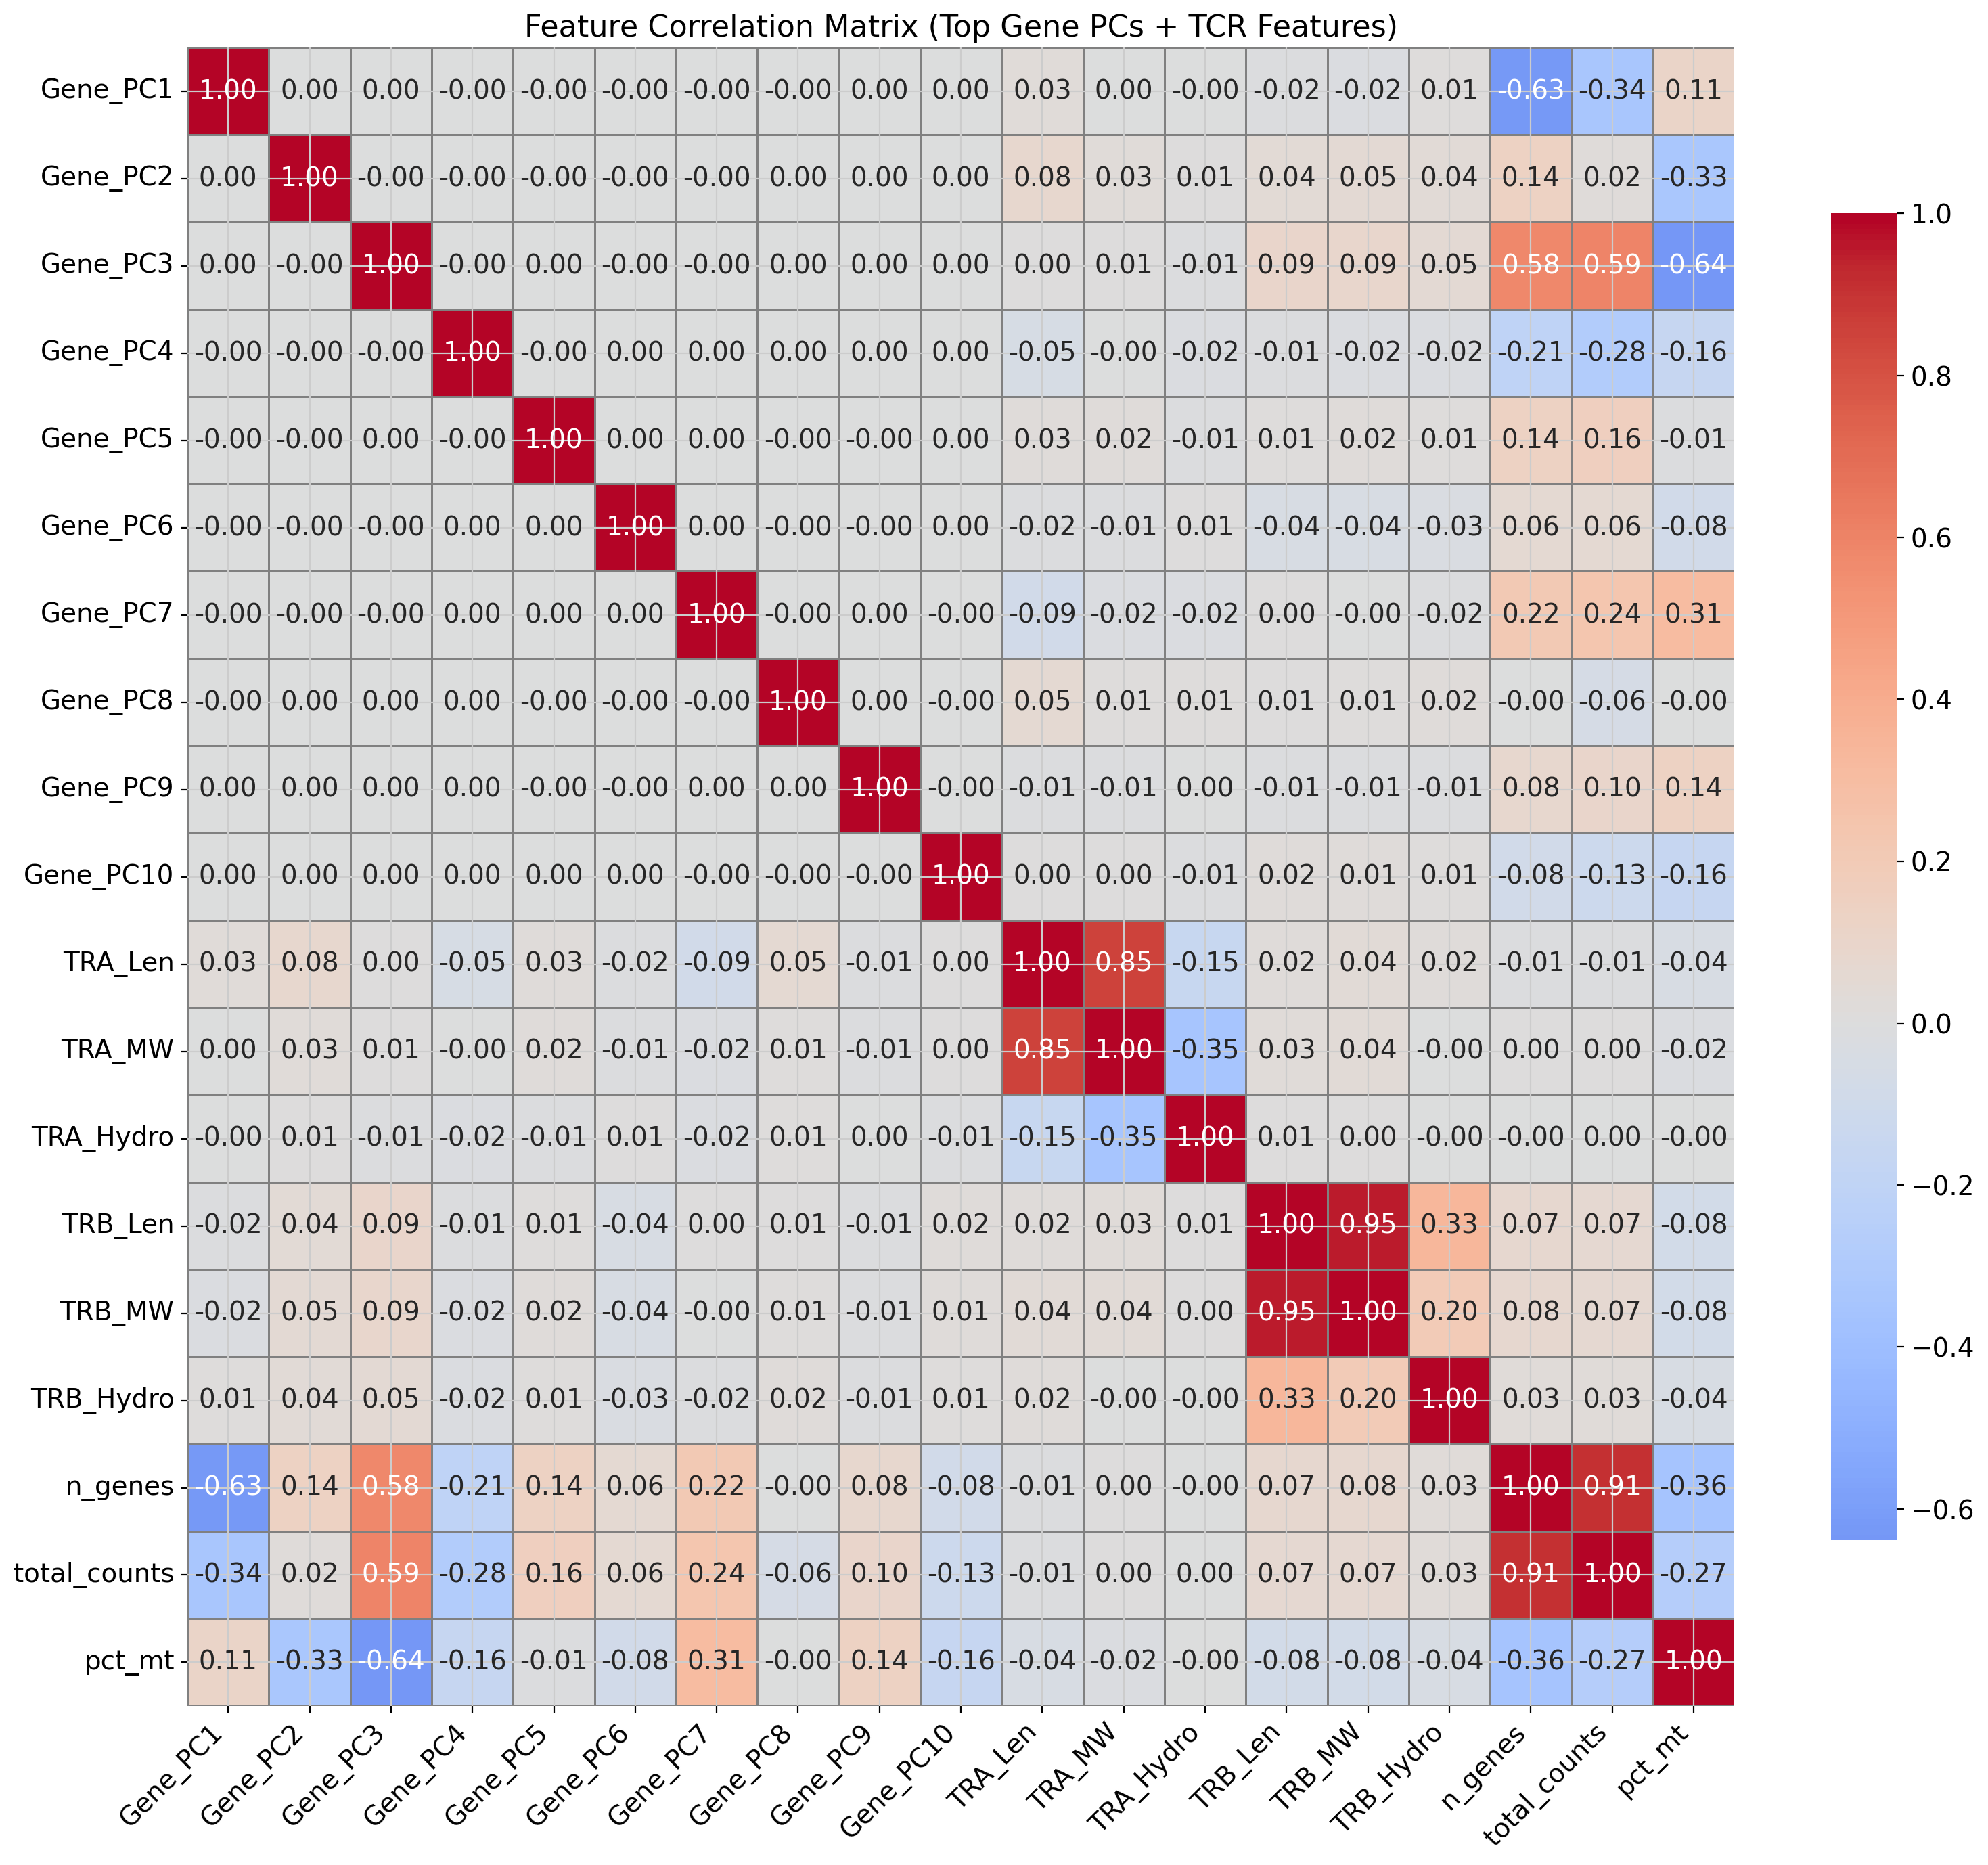
\includegraphics{Feature_Heatmappng.png}}
    \caption{Pearson correlation matrix for the top engineered features (first 20 gene-expression PCs and select TCR/receptor summary statistics). Block-diagonal structure indicates orthogonality between transcriptomic and receptor feature families.}
  \end{subfigure}
  \vspace{10pt}
  \begin{subfigure}[b]{0.92\linewidth}
    \centering
    \adjustbox{max size={\linewidth}{\dimexpr0.42\textheight-15pt\relax}}{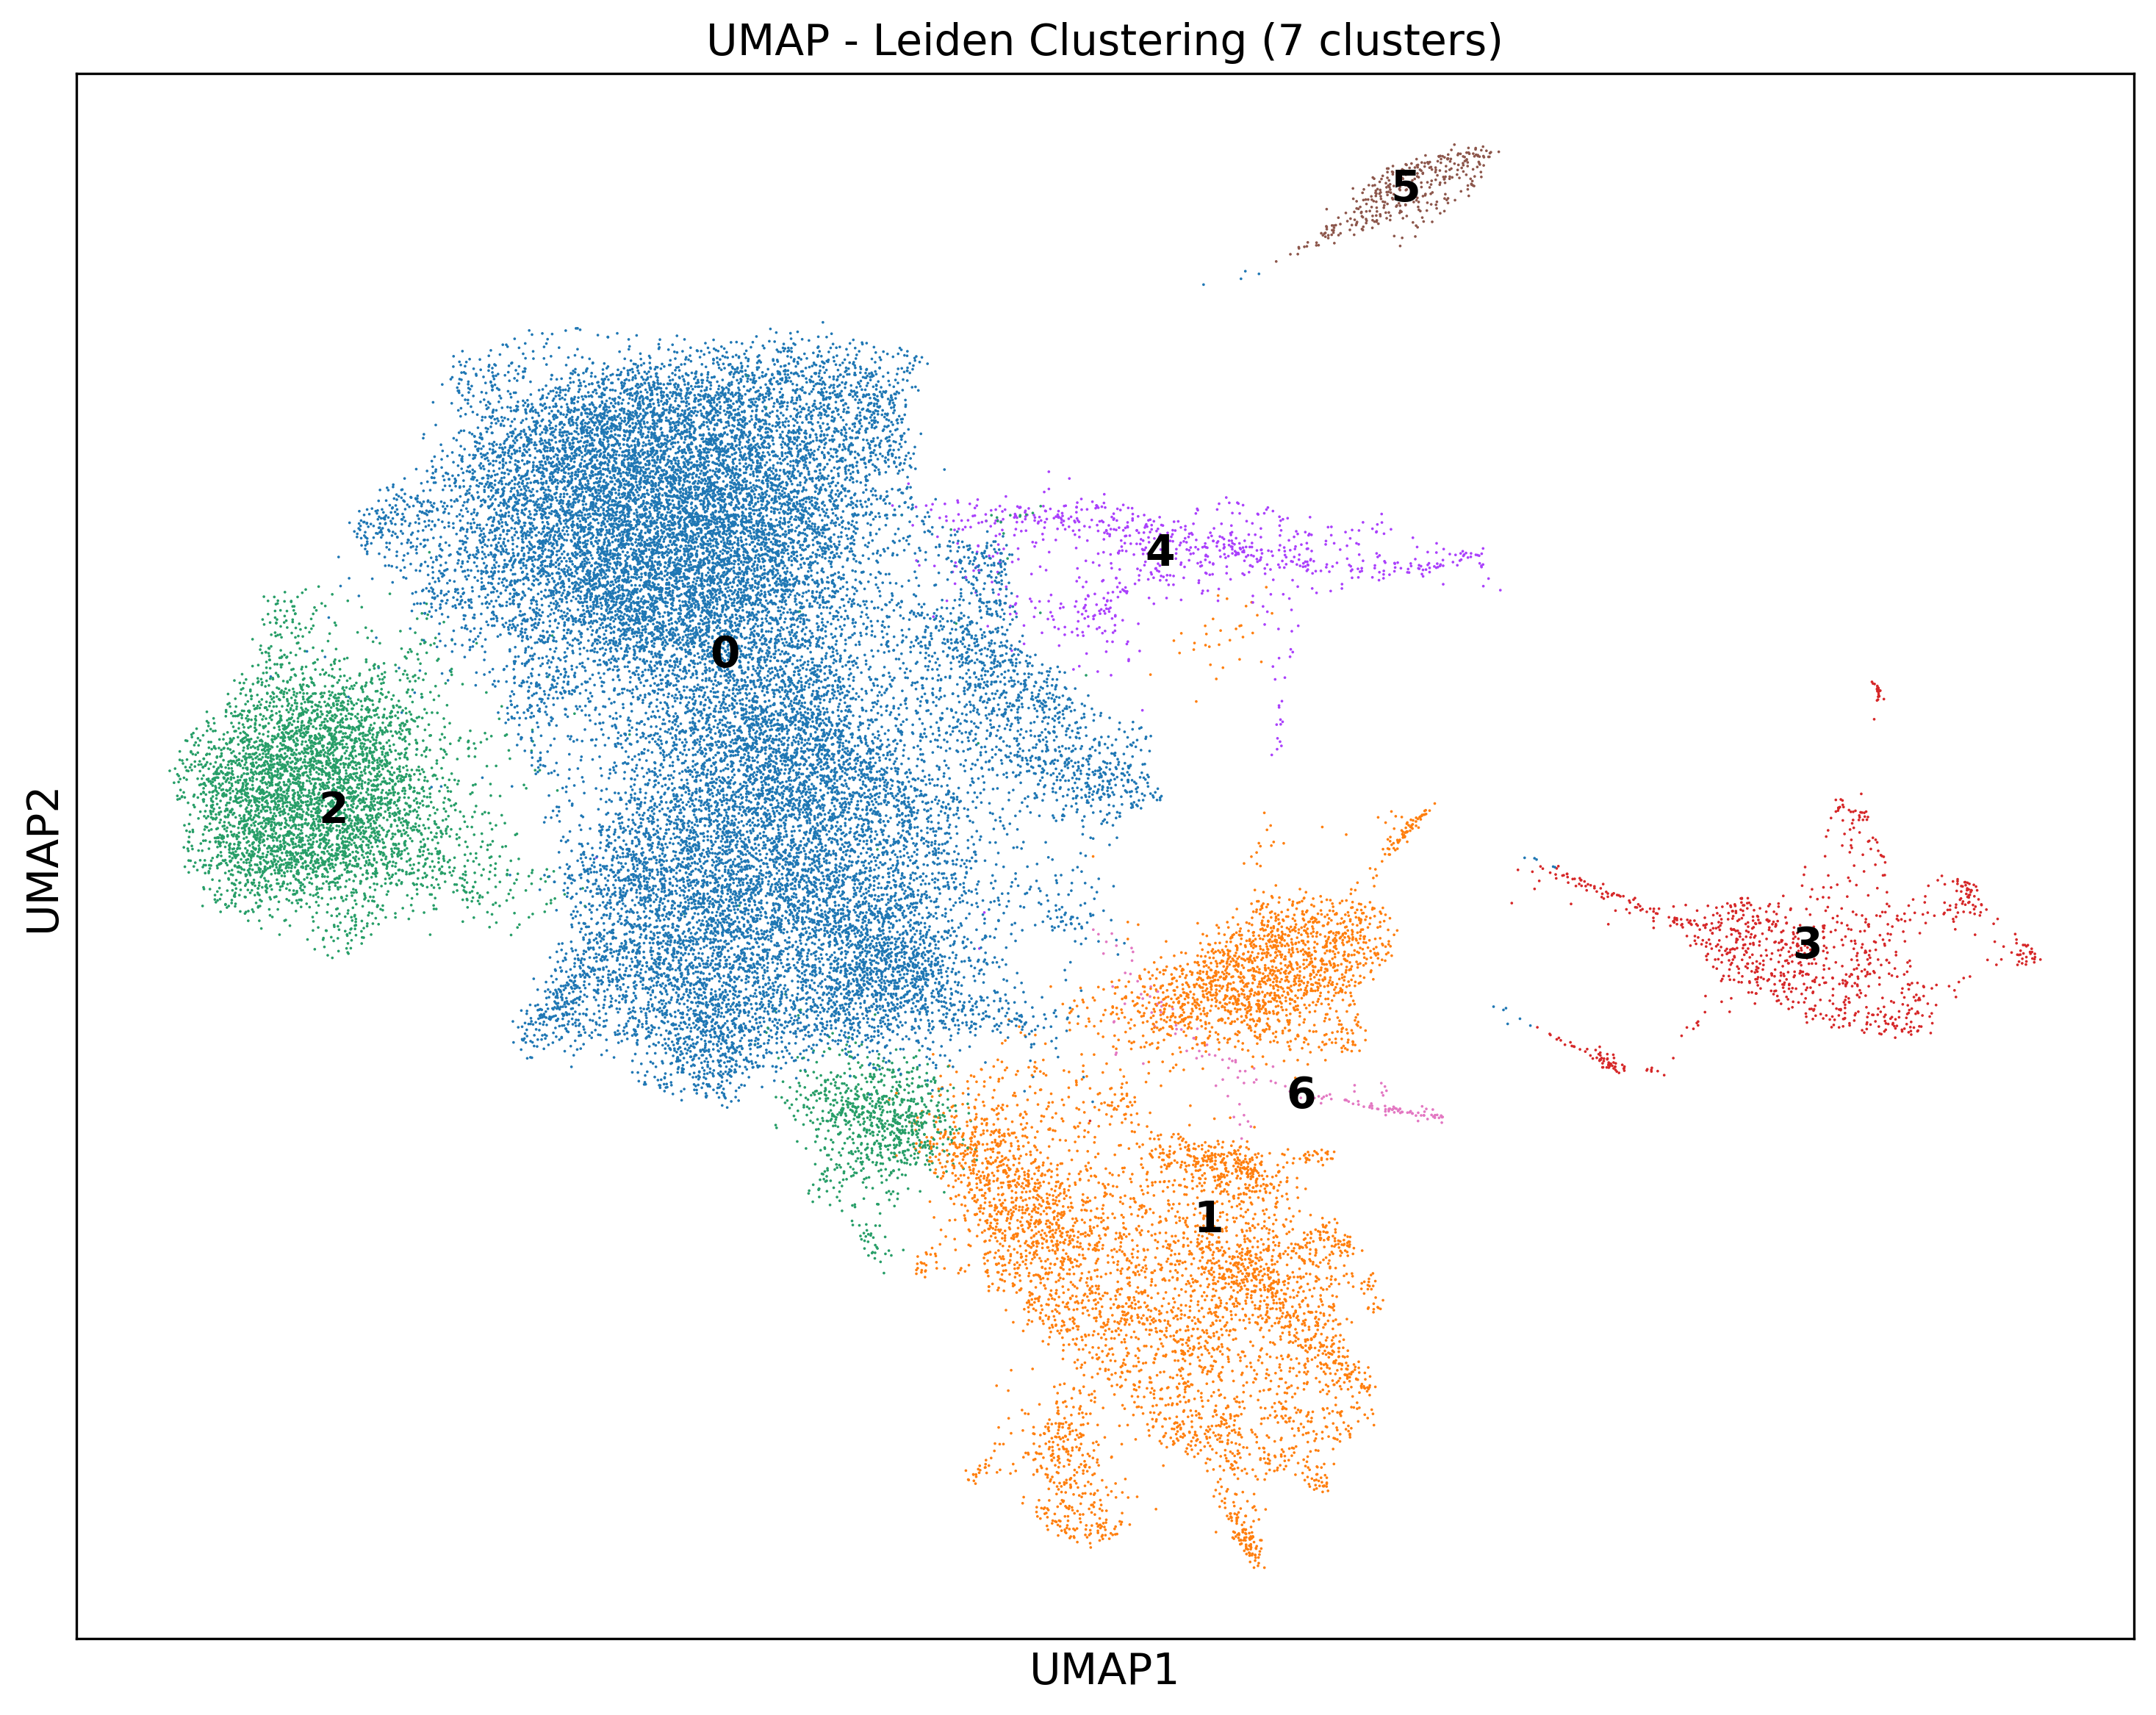
\includegraphics{umap_clusters.png}}
    \caption{UMAP visualization of peripheral blood immune cells colored by Leiden cluster assignment (7 clusters, silhouette-optimized). Distinct clusters capture heterogeneous immune cell states relevant to treatment response.}
  \end{subfigure}
  \vspace{6pt}
  \caption{Feature correlation structure and immune cell clustering. (a) The heatmap confirms low inter-family correlation, supporting the value of multimodal feature integration. (b) UMAP reveals well-separated immune subpopulations captured by the model.}
\end{figure}

\end{document}